% Options for packages loaded elsewhere
\PassOptionsToPackage{unicode}{hyperref}
\PassOptionsToPackage{hyphens}{url}
\PassOptionsToPackage{dvipsnames,svgnames,x11names}{xcolor}
%
\documentclass[
  letterpaper,
  DIV=11,
  numbers=noendperiod]{scrartcl}

\usepackage{amsmath,amssymb}
\usepackage{iftex}
\ifPDFTeX
  \usepackage[T1]{fontenc}
  \usepackage[utf8]{inputenc}
  \usepackage{textcomp} % provide euro and other symbols
\else % if luatex or xetex
  \usepackage{unicode-math}
  \defaultfontfeatures{Scale=MatchLowercase}
  \defaultfontfeatures[\rmfamily]{Ligatures=TeX,Scale=1}
\fi
\usepackage{lmodern}
\ifPDFTeX\else  
    % xetex/luatex font selection
\fi
% Use upquote if available, for straight quotes in verbatim environments
\IfFileExists{upquote.sty}{\usepackage{upquote}}{}
\IfFileExists{microtype.sty}{% use microtype if available
  \usepackage[]{microtype}
  \UseMicrotypeSet[protrusion]{basicmath} % disable protrusion for tt fonts
}{}
\makeatletter
\@ifundefined{KOMAClassName}{% if non-KOMA class
  \IfFileExists{parskip.sty}{%
    \usepackage{parskip}
  }{% else
    \setlength{\parindent}{0pt}
    \setlength{\parskip}{6pt plus 2pt minus 1pt}}
}{% if KOMA class
  \KOMAoptions{parskip=half}}
\makeatother
\usepackage{xcolor}
\setlength{\emergencystretch}{3em} % prevent overfull lines
\setcounter{secnumdepth}{-\maxdimen} % remove section numbering
% Make \paragraph and \subparagraph free-standing
\ifx\paragraph\undefined\else
  \let\oldparagraph\paragraph
  \renewcommand{\paragraph}[1]{\oldparagraph{#1}\mbox{}}
\fi
\ifx\subparagraph\undefined\else
  \let\oldsubparagraph\subparagraph
  \renewcommand{\subparagraph}[1]{\oldsubparagraph{#1}\mbox{}}
\fi


\providecommand{\tightlist}{%
  \setlength{\itemsep}{0pt}\setlength{\parskip}{0pt}}\usepackage{longtable,booktabs,array}
\usepackage{calc} % for calculating minipage widths
% Correct order of tables after \paragraph or \subparagraph
\usepackage{etoolbox}
\makeatletter
\patchcmd\longtable{\par}{\if@noskipsec\mbox{}\fi\par}{}{}
\makeatother
% Allow footnotes in longtable head/foot
\IfFileExists{footnotehyper.sty}{\usepackage{footnotehyper}}{\usepackage{footnote}}
\makesavenoteenv{longtable}
\usepackage{graphicx}
\makeatletter
\def\maxwidth{\ifdim\Gin@nat@width>\linewidth\linewidth\else\Gin@nat@width\fi}
\def\maxheight{\ifdim\Gin@nat@height>\textheight\textheight\else\Gin@nat@height\fi}
\makeatother
% Scale images if necessary, so that they will not overflow the page
% margins by default, and it is still possible to overwrite the defaults
% using explicit options in \includegraphics[width, height, ...]{}
\setkeys{Gin}{width=\maxwidth,height=\maxheight,keepaspectratio}
% Set default figure placement to htbp
\makeatletter
\def\fps@figure{htbp}
\makeatother

\KOMAoption{captions}{tableheading}
\makeatletter
\makeatother
\makeatletter
\makeatother
\makeatletter
\@ifpackageloaded{caption}{}{\usepackage{caption}}
\AtBeginDocument{%
\ifdefined\contentsname
  \renewcommand*\contentsname{Table of contents}
\else
  \newcommand\contentsname{Table of contents}
\fi
\ifdefined\listfigurename
  \renewcommand*\listfigurename{List of Figures}
\else
  \newcommand\listfigurename{List of Figures}
\fi
\ifdefined\listtablename
  \renewcommand*\listtablename{List of Tables}
\else
  \newcommand\listtablename{List of Tables}
\fi
\ifdefined\figurename
  \renewcommand*\figurename{Figure}
\else
  \newcommand\figurename{Figure}
\fi
\ifdefined\tablename
  \renewcommand*\tablename{Table}
\else
  \newcommand\tablename{Table}
\fi
}
\@ifpackageloaded{float}{}{\usepackage{float}}
\floatstyle{ruled}
\@ifundefined{c@chapter}{\newfloat{codelisting}{h}{lop}}{\newfloat{codelisting}{h}{lop}[chapter]}
\floatname{codelisting}{Listing}
\newcommand*\listoflistings{\listof{codelisting}{List of Listings}}
\makeatother
\makeatletter
\@ifpackageloaded{caption}{}{\usepackage{caption}}
\@ifpackageloaded{subcaption}{}{\usepackage{subcaption}}
\makeatother
\makeatletter
\@ifpackageloaded{tcolorbox}{}{\usepackage[skins,breakable]{tcolorbox}}
\makeatother
\makeatletter
\@ifundefined{shadecolor}{\definecolor{shadecolor}{rgb}{.97, .97, .97}}
\makeatother
\makeatletter
\makeatother
\makeatletter
\makeatother
\ifLuaTeX
  \usepackage{selnolig}  % disable illegal ligatures
\fi
\IfFileExists{bookmark.sty}{\usepackage{bookmark}}{\usepackage{hyperref}}
\IfFileExists{xurl.sty}{\usepackage{xurl}}{} % add URL line breaks if available
\urlstyle{same} % disable monospaced font for URLs
\hypersetup{
  pdftitle={GeographeAMP-report},
  pdfauthor={Claude Spencer, Brooke Gibbons, Tim Langlois},
  colorlinks=true,
  linkcolor={blue},
  filecolor={Maroon},
  citecolor={Blue},
  urlcolor={Blue},
  pdfcreator={LaTeX via pandoc}}

\title{GeographeAMP-report}
\author{Claude Spencer, Brooke Gibbons, Tim Langlois}
\date{}

\begin{document}
\maketitle
\ifdefined\Shaded\renewenvironment{Shaded}{\begin{tcolorbox}[frame hidden, sharp corners, interior hidden, borderline west={3pt}{0pt}{shadecolor}, breakable, enhanced, boxrule=0pt]}{\end{tcolorbox}}\fi

\hypertarget{existing-knowledge}{%
\section{Existing knowledge}\label{existing-knowledge}}

\hypertarget{background}{%
\subsection{Background}\label{background}}

\hypertarget{features-and-values-of-the-geographe-marine-park}{%
\subsection{Features and values of the Geographe Marine
Park}\label{features-and-values-of-the-geographe-marine-park}}

\begin{figure}

{\centering 
\includegraphics{images/GeographeAMP-broad-site-plot.png}

}

\caption{\label{fig-location}Study area of the Geographe Marine Park
showing the State and Commonwealth (Australian Marine Park) managed
marine park zones. The red line following the coast demarcates the
border of state and commonwealth waters. Bathymetric contours shown are
30, 70, 200 \& 700 m, which denote historical sea levels and ecosystem
depth contours.}

\end{figure}

\begin{figure}

{\centering 
\includegraphics{images/GeographeAMP-key-ecological-features.png}

}

\caption{\label{fig-kef}Key Ecological Features at the scale of the
Geographe Marine Park. Excerpt from Marine Key Ecological Features of
the Australian Marine Parks. Legend for Australian Marine Parks,
Terrestrial Managed Areas and State Marine Parks can be found in Figure
1. The red line delimits state and commonwealth waters. Geographe Bay =
Commonwealth marine environment within and adjacent to Geographe Bay,
Ancient coastline = Ancient coastline at 90-120m depth.}

\end{figure}

\begin{figure}

{\centering 
\includegraphics{images/GeographeAMP-old-sea-levels.png}

}

\caption{\label{fig-sealevels}Old coastline features of the Geographe
Marine Park. The dashed line represents the location of Figure X}

\end{figure}

\hypertarget{pressures}{%
\subsection{Pressures}\label{pressures}}

\hypertarget{latest-survey-aims-design-and-methods}{%
\section{Latest survey aims, design and
methods}\label{latest-survey-aims-design-and-methods}}

\hypertarget{aims-and-objectives}{%
\subsection{Aims and objectives}\label{aims-and-objectives}}

\hypertarget{discovery-questions-interaction-of-environmental-values-and-pressures-rationale-for-future-surveys-and-monitoring}{%
\subsection{Discovery questions: interaction of environmental values and
pressures, rationale for future surveys and
monitoring}\label{discovery-questions-interaction-of-environmental-values-and-pressures-rationale-for-future-surveys-and-monitoring}}

\hypertarget{survey-design}{%
\subsection{Survey design}\label{survey-design}}

\hypertarget{survey-stages}{%
\subsection{Survey stages}\label{survey-stages}}

\begin{figure}

{\centering 
\includegraphics{images/GeographeAMP-sampling-locations.png}

}

\caption{\label{fig-sites}Sampling locations in the Geographe Marine
Park. The red boundary following the coast demarcates State waters, and
depth contours represent the 30 m ecosystem depth contour.}

\end{figure}

\hypertarget{latest-results-and-discussion}{%
\section{Latest results and
discussion}\label{latest-results-and-discussion}}

\hypertarget{bathymetry-and-relief}{%
\subsection{Bathymetry and relief}\label{bathymetry-and-relief}}

\hypertarget{bathymetry-and-significant-seafloor-features}{%
\subsubsection{Bathymetry and significant seafloor
features}\label{bathymetry-and-significant-seafloor-features}}

\begin{figure}

{\centering 
\includegraphics{images/GeographeAMP-bathymetry-cross-section.png}

}

\caption{\label{fig-cross}Transect across significant seafloor and
submerged coastal features across the Ngari Capes Marine Park and GMP.
Submerged coastlines from thousands of years before present (Ka BP) are
indicated. The red line delimits State and Commonwealth waters. The
green and pale blue line delimits the National Park Zone and GMP limit
respectively. Distances from the coast are measured in km. The location
of this transect is given in Figure X.}

\end{figure}

\hypertarget{benthic-biota-and-habitat-extent}{%
\subsection{Benthic biota and habitat
extent}\label{benthic-biota-and-habitat-extent}}

\hypertarget{distribution-of-dominant-habitat-classes}{%
\subsubsection{Distribution of dominant habitat
classes}\label{distribution-of-dominant-habitat-classes}}

\hypertarget{broader-study-area---habitat-extent}{%
\subsubsection{Broader study area - habitat
extent}\label{broader-study-area---habitat-extent}}

\hypertarget{characterization-of-significant-seafloor-features}{%
\subsubsection{Characterization of significant seafloor
features}\label{characterization-of-significant-seafloor-features}}

\hypertarget{fish-assemblage}{%
\subsection{Fish assemblage}\label{fish-assemblage}}

\hypertarget{broader-study-area}{%
\subsubsection{Broader study area}\label{broader-study-area}}

\begin{figure}

{\centering 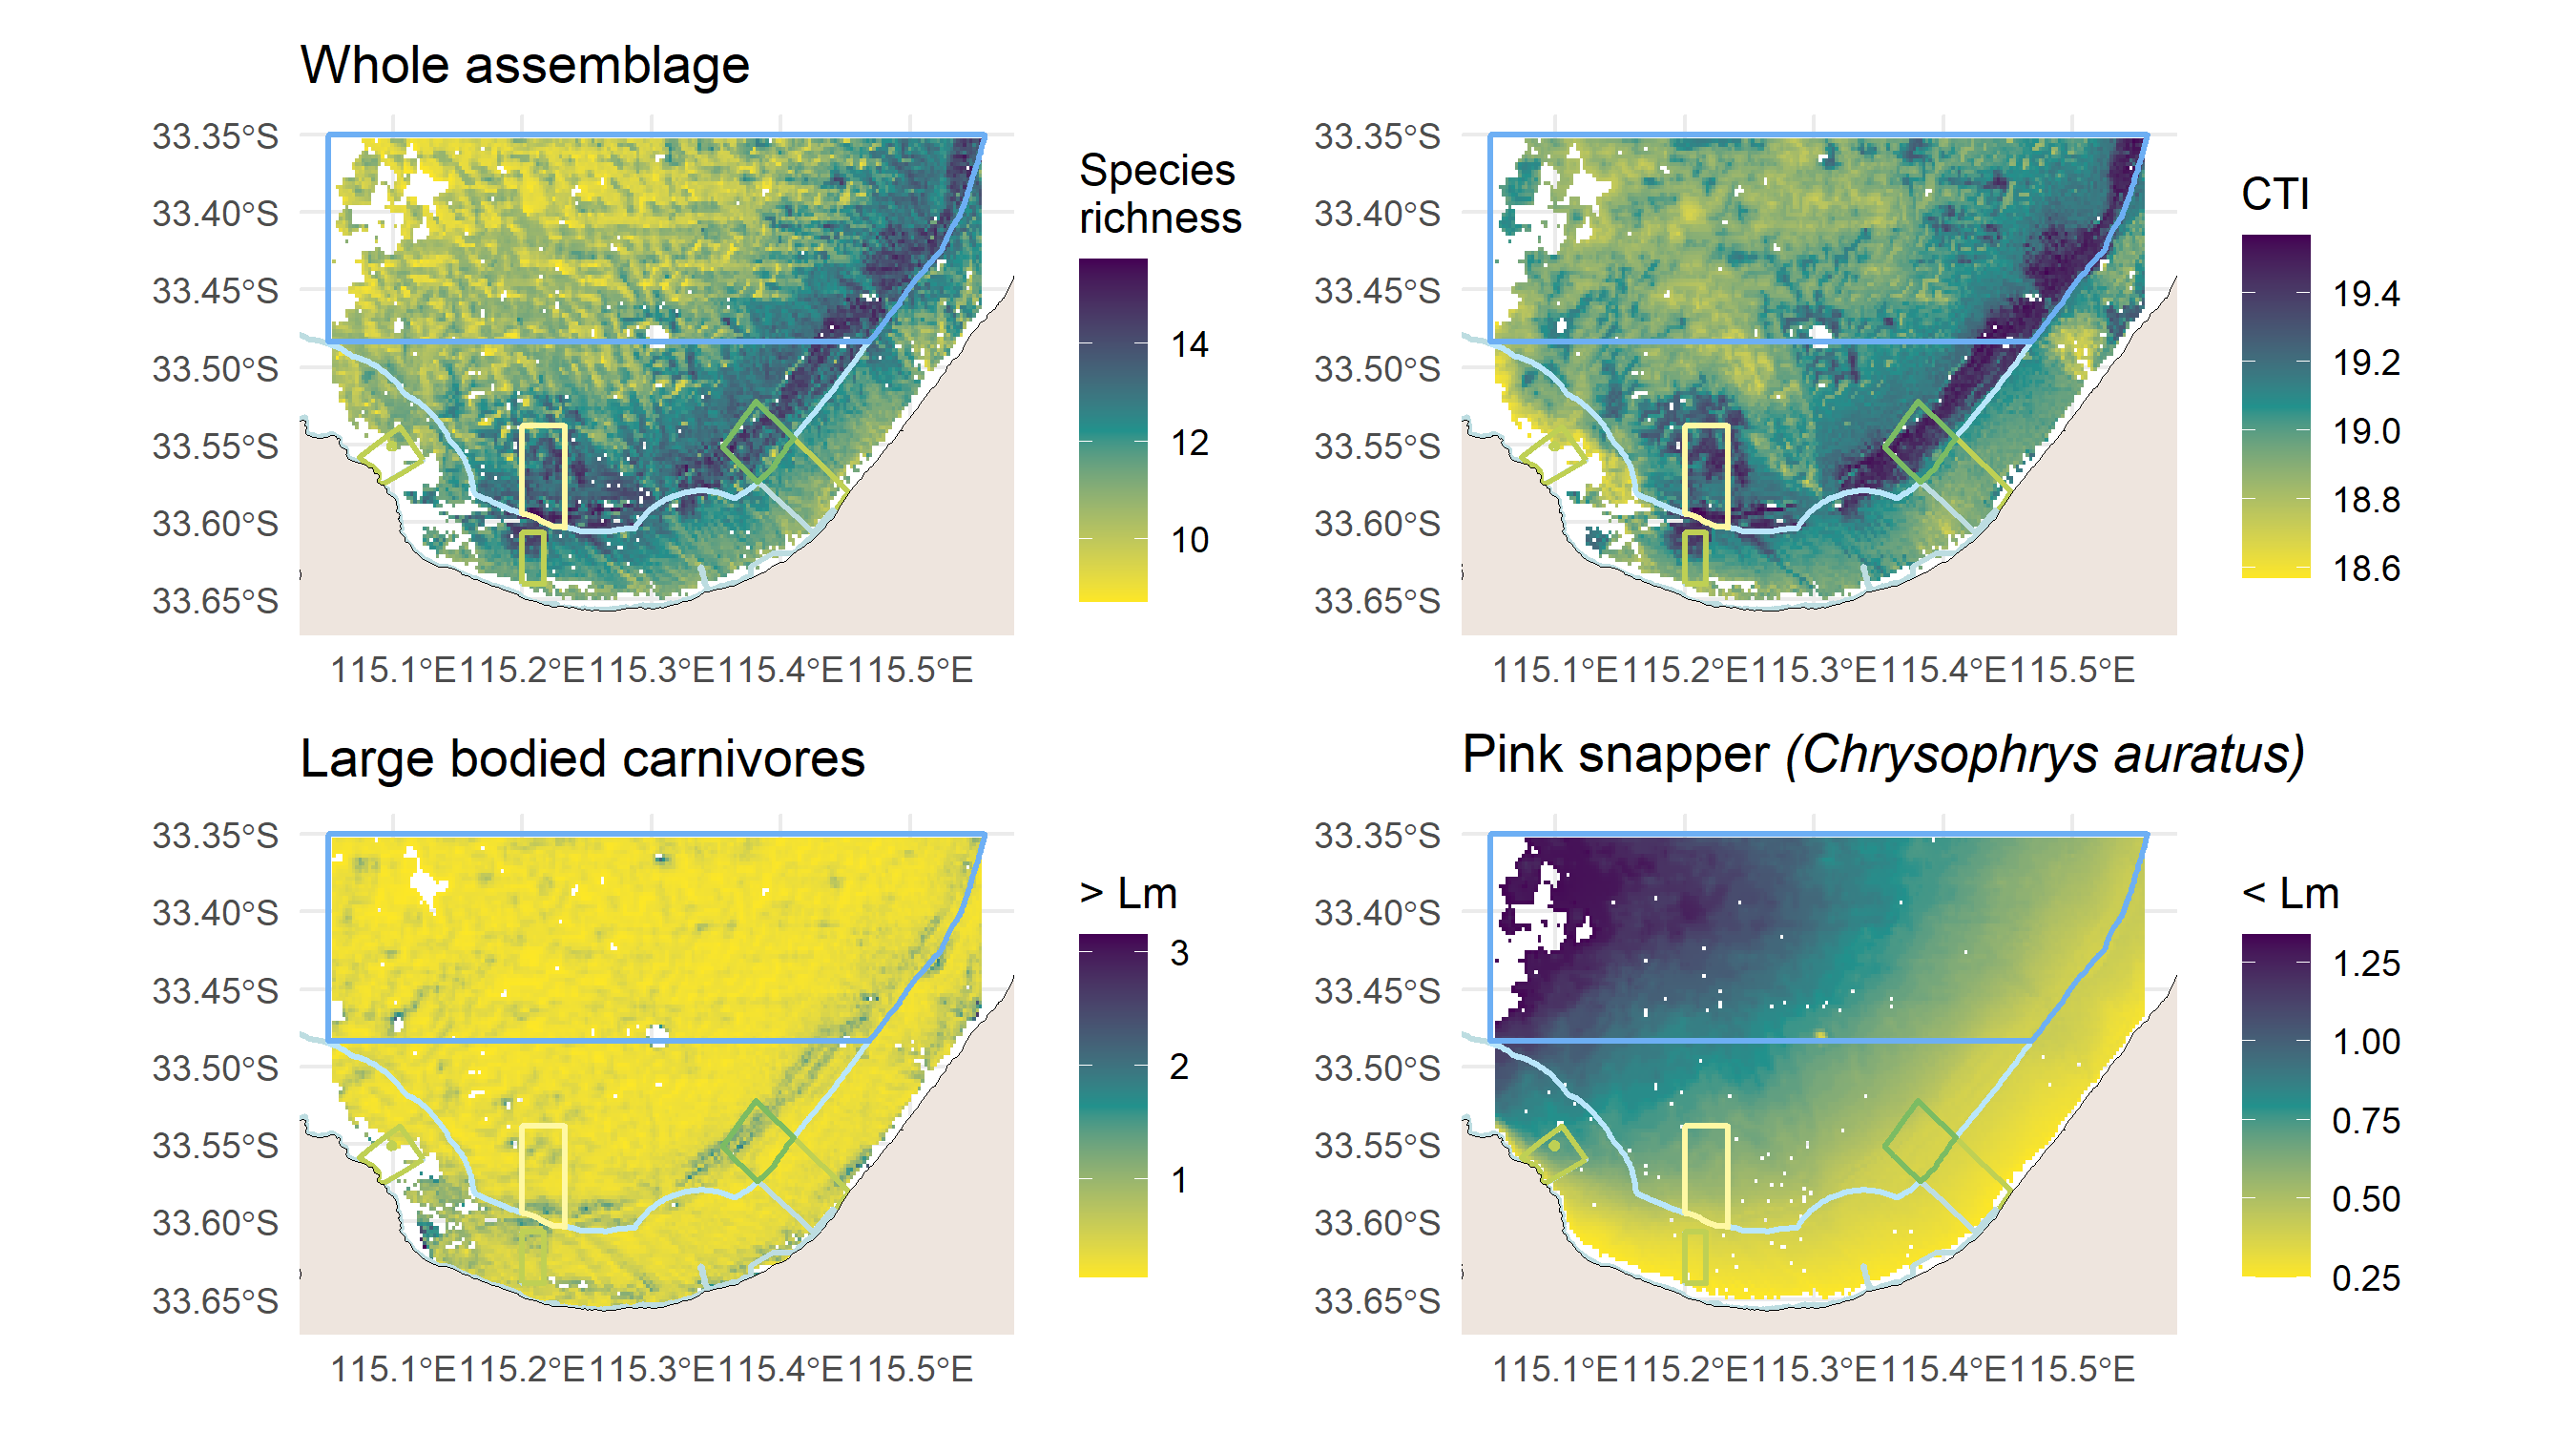
\includegraphics{images/GeographeAMP_fish-individual_predictions.png}

}

\caption{\label{fig-spatialpreds}Spatial predictions of key fish metrics
for the Geographe Marine Park.}

\end{figure}

Spatial patterns in the distribution of key fish metrics for the
Geographe Marine Park highlight increased species richness along reef
features that run through the National Park and Habitat Protection Zones
(Figure~\ref{fig-spatialpreds}).

\begin{figure}

{\centering 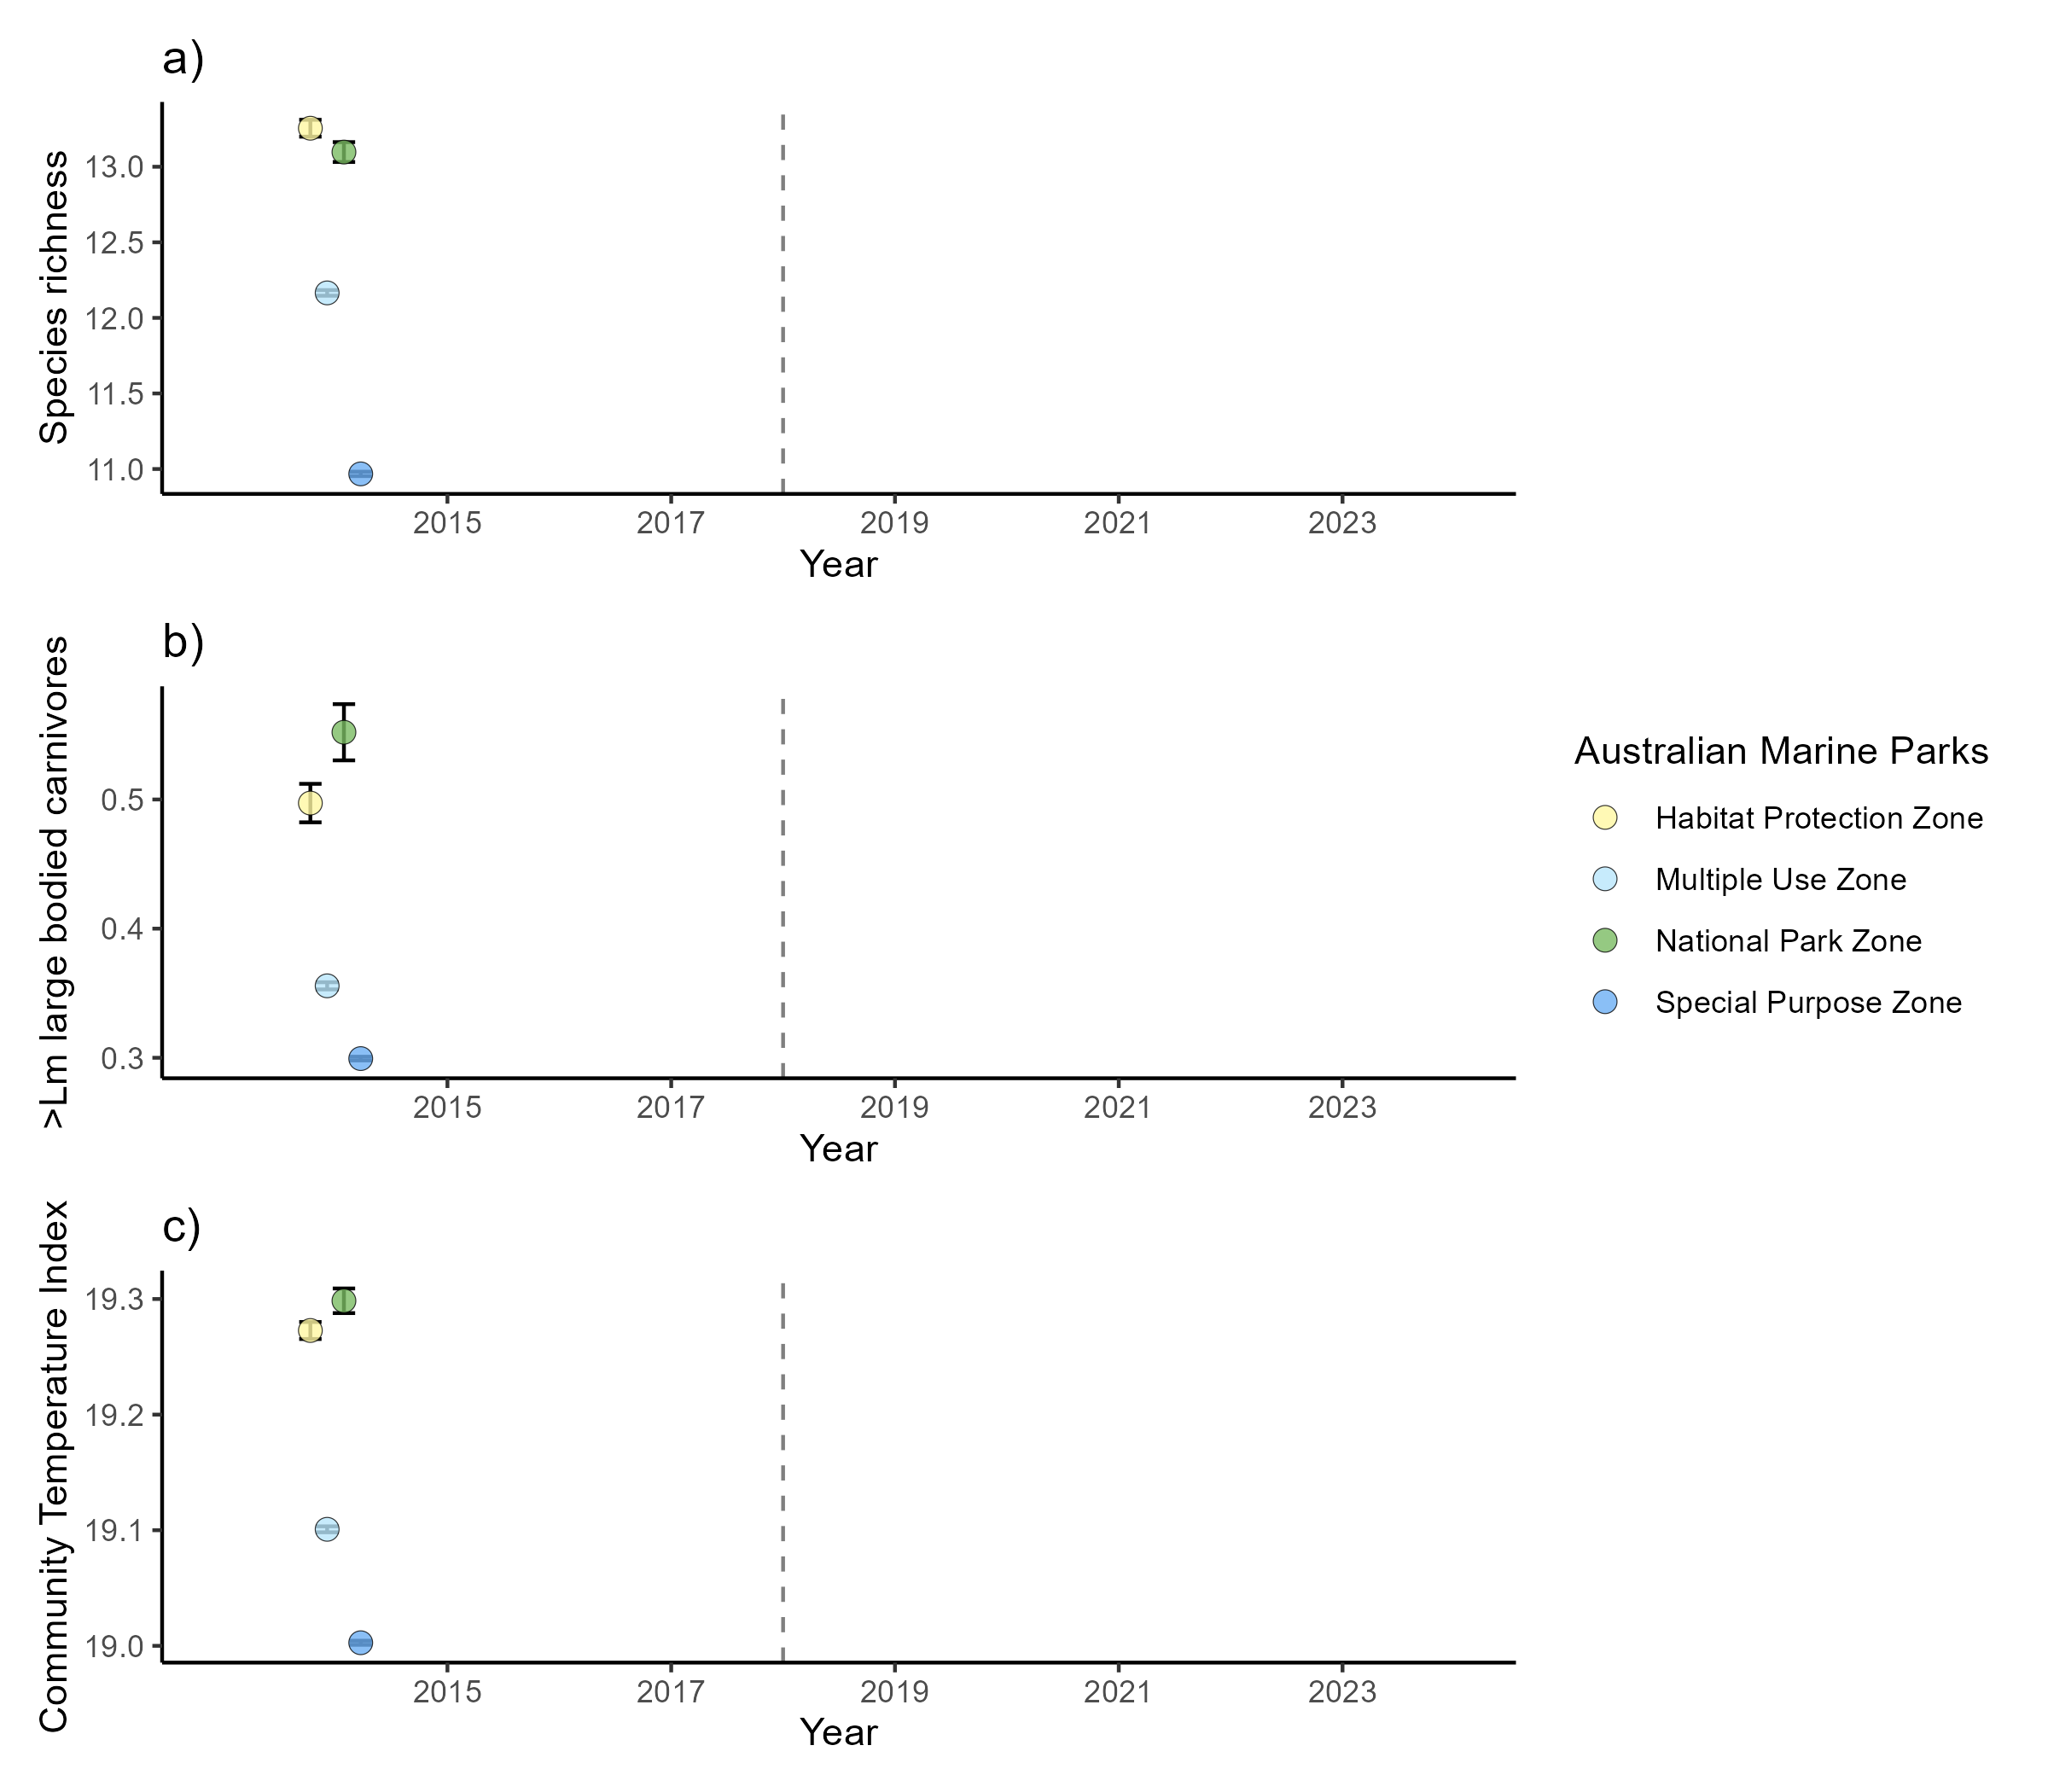
\includegraphics{images/GeographeAMP_control-plots.png}

}

\caption{\label{fig-temppreds}Temporal predictions of key fish metrics
for the Geographe Marine Park.}

\end{figure}

Temporal trends of key fish metrics for the Geographe Marine Park
highlight increased abundance of mature large bodied carnivorous species
in the National Park Zone (Figure~\ref{fig-temppreds}).

\hypertarget{threatened-species}{%
\subsubsection{Threatened species}\label{threatened-species}}

\hypertarget{general-conclusions-and-recommendations-for-future-work}{%
\section{General conclusions and recommendations for future
work}\label{general-conclusions-and-recommendations-for-future-work}}

\hypertarget{general-conclusions}{%
\subsection{General conclusions}\label{general-conclusions}}

\hypertarget{recommendations-for-benchmarks-and-monitoring}{%
\subsection{Recommendations for benchmarks and
monitoring}\label{recommendations-for-benchmarks-and-monitoring}}

\hypertarget{guidance-for-future-studies-and-surveys}{%
\subsection{Guidance for future studies and
surveys}\label{guidance-for-future-studies-and-surveys}}

\hypertarget{references}{%
\section{References}\label{references}}



\end{document}
